\documentclass[11pt,a4paper]{report}
\usepackage{graphicx}
\usepackage[utf8]{inputenc}
%\usepackage[english]{babel}
\usepackage[portuguese]{babel}
\usepackage[margin=2.5cm]{geometry}
%\usepackage[toc,page]{appendix}
\usepackage[nottoc,numbib]{tocbibind}
\usepackage{pdfpages}
\usepackage{parskip}
\usepackage{url}
\usepackage{xurl}
\usepackage{array}
\usepackage[acronym, nonumberlist]{glossaries}
\usepackage[hidelinks]{hyperref}
\usepackage{float}
\usepackage{times}
\usepackage{etoolbox}
\makeatletter
\renewcommand\footnotesize{\@setfontsize\footnotesize{9pt}{9pt}\fontfamily{ptm}\selectfont}
\makeatother
\usepackage[font=footnotesize,labelfont=bf]{caption}
\usepackage{setspace}
\onehalfspacing
\makeglossaries
\usepackage{listings}
\renewcommand{\lstlistingname}{Lista}
\renewcommand*{\lstlistlistingname}{Lista de Listagens}
\lstset{
 xleftmargin = 1cm,
 basicstyle=\footnotesize, 
 numbers=left, 
 captionpos=b,
 columns=fullflexible,
 breaklines=true,
 frame=single
}

\begin{document}
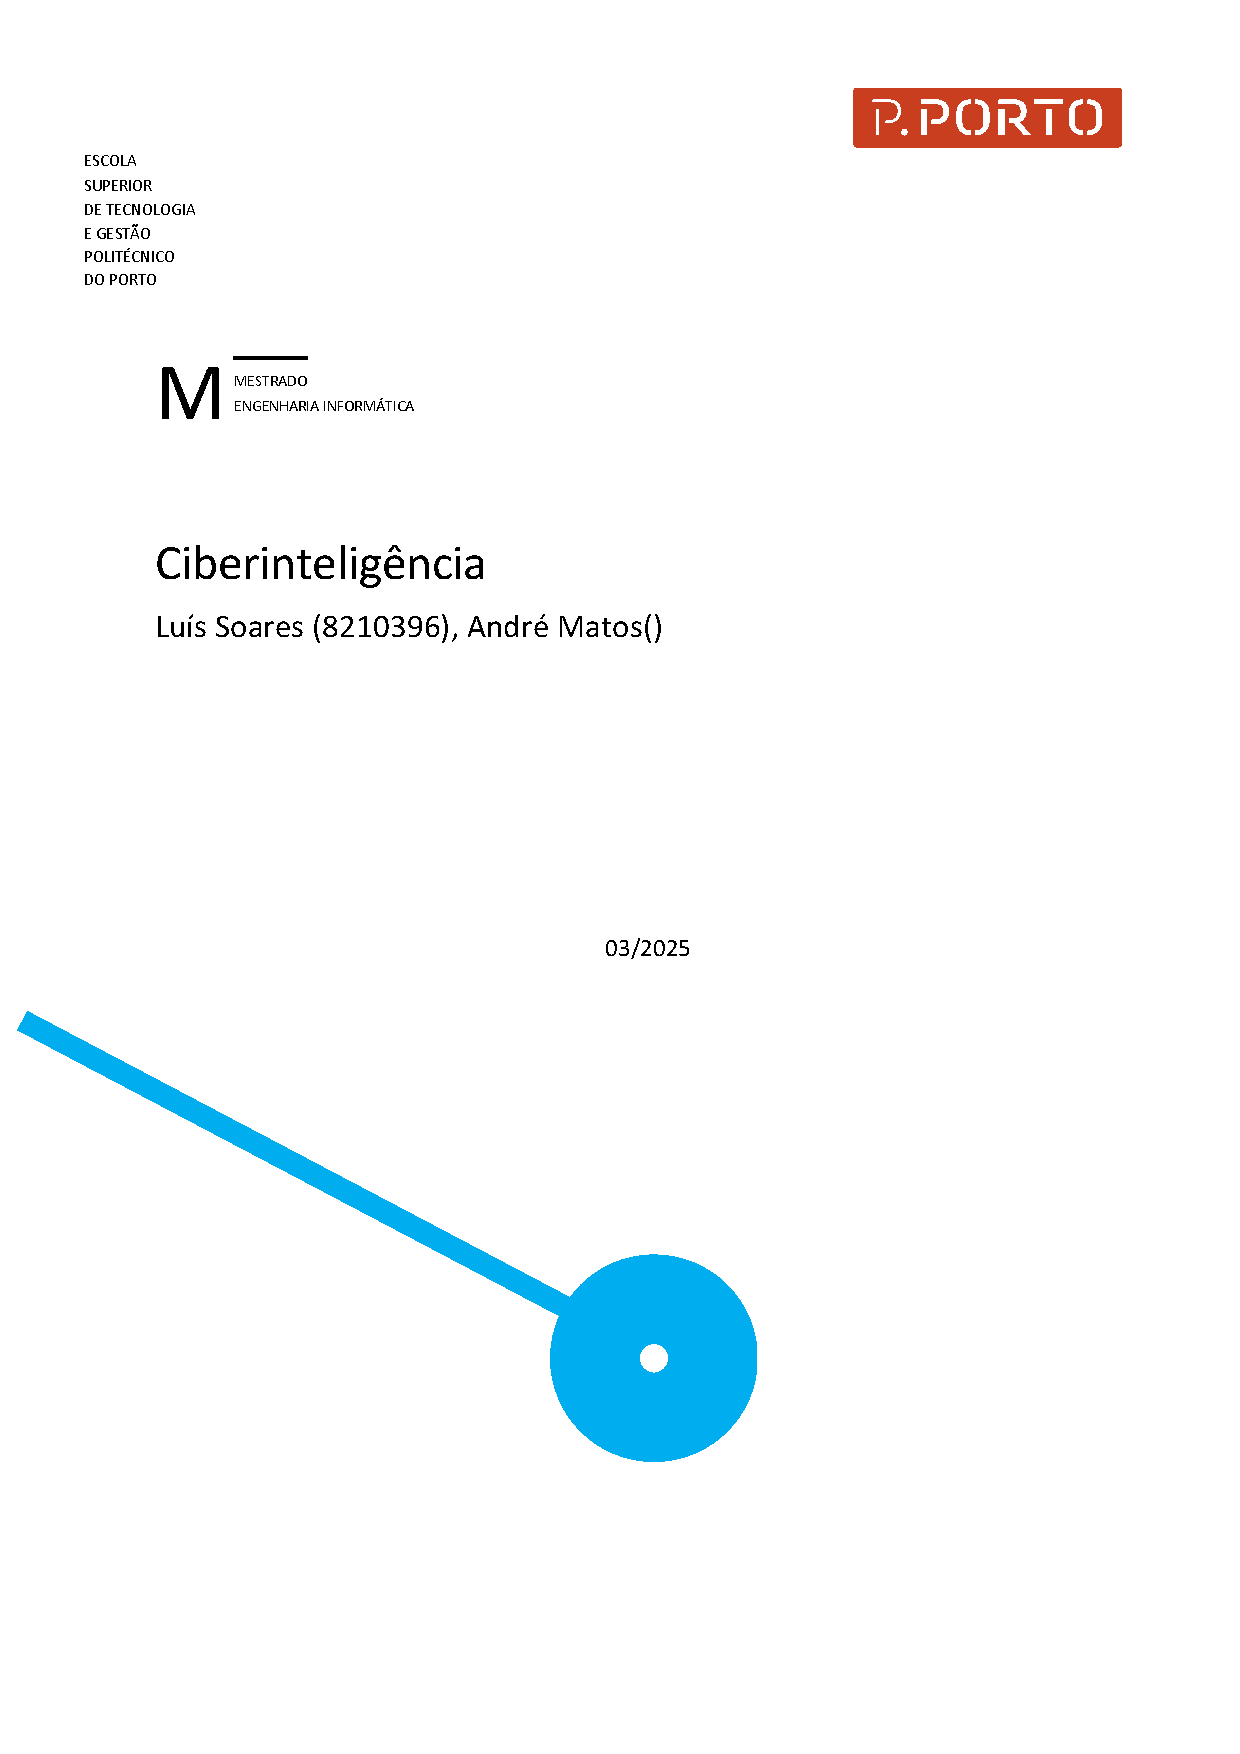
\includepdf[pages=1-2]{cover/cover.pdf}
\pagenumbering{roman}
\newacronym{estg}{ESTG}{Escola Superior de Tecnologia e Gestão}
\newacronym{ipp}{IPP}{Instituto Politécnico do Porto}


\chapter*{Declaração de integridade}

Nós, \textbf{Luís Soares}, estudante nº \textbf{8210396}, e \textbf{Luís Soares}, estudante nº \textbf{8210396} do Mestrado \textbf{Engenharia Informática} da Escola Superior de Tecnologia e Gestão do Instituto Politécnico do Porto, declaro que não fizemos plágio nem auto-plágio, pelo que o trabalho intitulado “\textbf{TODO: Change This}” é original e da nossa autoria, não tendo sido usado previamente para qualquer outro fim. Mais declaramos que todas as fontes usadas estão citadas, no texto e na bibliografia final, segundo as regras de referenciação adotadas na instituição.

\chapter*{Agradecimentos}

Gostaríamos de expressar a nossa gratidão ao Professor Doutor Davide Rua Carneiro pela
orientação, apoio e paciência durante o desenvolvimento deste trabalho.
Toda a experiência e conhecimento foram essenciais para a realização deste projeto.

Agradecemos também aos nossos colegas de curso pela troca de conhecimentos,
experiências e pelo espírito de camaradagem que sempre nos motivou a continuar,
mesmo nos momentos mais desafiadores.

Aos nossos familiares, pelo suporte incondicional, compreensão e encorajamento ao
longo desta jornada académica. Sem o vosso apoio, este trabalho não teria sido possível.

Por fim, agradecemos a todos que, direta ou indiretamente, contribuíram para a
realização deste trabalho. A todos, o nosso sincero obrigado.

\chapter*{Abstract}



\textbf{Keywords:} 

\chapter*{Resumo}



\textbf{Palavras-chave:} 

\tableofcontents

\listoffigures

\listoftables

\addcontentsline{toc}{chapter}{Lista de Listagens}
\lstlistoflistings

\printglossary[type=\acronymtype,title=Lista de Acrónimos]
\addcontentsline{toc}{chapter}{Lista de Acrónimos}

%#region Introdução

\chapter{Introdução}
\pagenumbering{arabic}
\cite{estg-website}

\section{Contextualização}

\section{Apresentação do Caso de Estudo}

\section{Motivação e Objetivos}

\textbf{Motivação:}


\textbf{Objetivos:}


\section{Estrutura do Relatório}

O presente relatório está organizado da seguinte forma:

%#endregion

\chapter{Caracterização Geral do Problema}

Esta secção deve
incluir uma caracterização geral do problema bem como dos fatores mais relevantes
indicados na literatura. Deve apresentar um glossário com os principais termos do
domínio, bem como uma descrição das fontes de dados identificadas, que deve incluir, no
mínimo, uma descrição da forma de aceder aos dados, e um dicionário de dados (por fonte)

\section{\textit{Problem Description}}

\section{\textit{Business Glossary}}

\section{\textit{Data sources description}}

\chapter{...}

\section{\textit{Data description report}}

Esta secção, descreve o trabalho que ocorre após a integração dos
dados, e deve descrever o(s) dataset(s) resultante(s) e que serão usados como base para as
tarefas de processamento e análise de dados. Entre outros aspetos, esta secção deve pelo
menos analisar a quantidade e qualidade (e.g. distribuição das variáveis, dados em falta,
problemas nos dados e tarefas de limpeza necessárias) dos dados disponíveis. Isto será
usado como base para o trabalho a desenvolver na fase seguinte.

\section{\textit{Data processing report}}

Esta secção deve descrever todas as tarefas de limpeza,
transformação, criação (feature engineering), ou outras levadas a cabo de forma a melhorar
a qualidade dos dados, e a expor da melhor forma o conhecimento existente para a fase de
Machine Learning que se segue.

\chapter{Machine Learning}

Esta secção deve descrever as tarefas de modelação levadas a cabo,
bem como uma análise crítica dos seus resultados. Ou seja, deve ser possível perceber pela
leitura desta secção, que algoritmos foram utilizados, que modelos foram produzidos e qual
a sua qualidade, como os modelos foram produzidos e avaliados, ou ainda qual ou quais os
modelos selecionados para colocar em produção no dashboard.

\chapter{Conclusões e Trabalho Futuro}

<<Elaborar uma apreciação crítica sobre o trabalho realizado, apontando os seus pontos fortes e fracos. Adicionalmente, caso se aplique, enunciar eventuais tarefas a realizar futuramente ou novas opções para estender o trabalho realizado.>>

\bibliographystyle{ieeetr}
\bibliography{refs}

\appendix



\end{document}
